\subsection{Fourier series}
Instead of arbitrary $\phi_i$ substitute $e^{i \pi k}$ to \eqref{eq:linear_expansion}:
\begin{equation*}
	\begin{multlined}
		S_K(x) = \beta_0 + \sum_{i = 1}^K \beta_i e^{i \pi k x} \implies S(x) = a_0 + \sum_{i = 1}^K \left (a_i cos(\pi k x) + b_i sin(\pi k x) \right ) \\
	\end{multlined}
\end{equation*}
This set of functions is orthogonal on the considered interval:
\begin{equation*} 
	\int_{-\pi}^{\pi} e^{i \pi k x} e^{i \pi l x} = 2\pi \delta_k^l 
\end{equation*}
The estimation of $a_n$ and $b_n$ for some function $f$ is a straightforward process, first of all, define the residual for this expansion - $R(x) = f(x) - S_K(x)$, after that, integrate the squared residual over the domain and use the least-squares method:
\begin{equation*}
	\begin{multlined}
		\mathcal{L} = \int_{\Omega} R(x)^2 d\Omega = \int_{\Omega} \left ( f(x) - S_K(x) \right )^2 d\Omega = \\ = \int_{\Omega} f(x)^2 d\Omega - 2 \int_{\Omega} S_K(x) f(x) d\Omega + \int_{\Omega} S_K(x)^2 d\Omega = \\ = \int_{\Omega} f(x)^2 d\Omega - 2 \int_{\Omega} \left [ a_0 + \sum_{i = 1}^K \left (a_i cos(\pi k x) + b_i sin(\pi k x) \right ) \right ] f(x) d\Omega + \\ +  \int_{\Omega} \left [ a_0 + \sum_{i = 1}^K \left (a_i cos(\pi k x) + b_i sin(\pi k x) \right ) \right ]^2 d\Omega
	\end{multlined}
\end{equation*}
And the derivates of the integrated residual:
\begin{equation}
 	\begin{multlined}
 		\begin{cases}
 			\dfrac{\partial }{\partial a_n} \mathcal{L} = \dfrac{\partial \mathcal{L}}{\partial S_K(x)} \dfrac{\partial S_K(x)}{\partial a_n}  = -2 {\displaystyle \int_{\Omega}} f(x) cos(\pi k x) d\Omega + -2 {\displaystyle \int_{\Omega}} S_K(x) cos(\pi k x) d\Omega \\[20pt]
 			\dfrac{\partial }{\partial b_n} \mathcal{L} = \dfrac{\partial \mathcal{L}}{\partial S_K(x)} \dfrac{\partial S_K(x)}{\partial b_n} = -2 {\displaystyle \int_{\Omega}} f(x) sin(\pi k x) d\Omega + -2 {\displaystyle \int_{\Omega}} S_K(x) sin(\pi k x) d\Omega \\[20pt]
 			\dfrac{\partial }{\partial a_0} \mathcal{L} = \dfrac{\partial \mathcal{L}}{\partial S_K(x)} \dfrac{\partial S_K(x)}{\partial a_0}  = -2 {\displaystyle \int_{\Omega}} f(x) d\Omega + 2 |\Omega| a_0 \\[20pt]
 		\end{cases}
 	\end{multlined}
 	% \mathcal{L} = \int_{\Omega} R(x)^2 d\Omega
\end{equation}
The main part of the calculations is absent and provided here \cite{fourierintro}. In addition, there is a convergence analysis of the coefficients, in sense of pointwise, and $L_2$ norm. The final result for the coefficients is:
\begin{equation}
	\begin{cases}
		a_0 = \dfrac{{\displaystyle \int_{\Omega}} f(x) d\Omega }{2 | \Omega |} \\[20pt]
		a_n = \dfrac{{\displaystyle \int_{\Omega}} f(x) cos(\pi k x) d\Omega}{| \Omega |} \\[20pt]
		b_n = \dfrac{{\displaystyle \int_{\Omega}} f(x) sin(\pi k x) d\Omega}{| \Omega |} \\[20pt]
	\end{cases}
\end{equation}

\paragraph{Example of function expansion into the Fourier series} 
Consider the function $y = sin(x) + x$ and at the fig. \ref{fig:fourier_demo} the results. It can be seen that with a relatively small amount of the terms the approximation good. With 3 terms the approximation error\footnote{Here, the approximation error is the loss function and concrete - mean squared error between the known values and Fourier expansion. There is a pointwise loss value, where the error calculation includes the finite number of nodes and integral loss value, where the residual integrates over the all domain.} is 0.565, 5 terms - 0.005 and 10 terms is 0.002.
\begin{figure}[h]
	\centering
	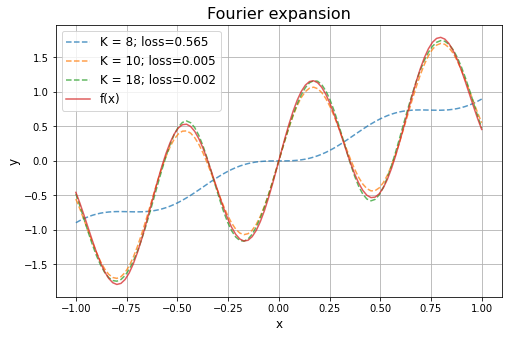
\includegraphics[width=0.65 \textwidth]{images/chapter2/fourier_demo.png}
	\caption{Example of function expansion into the Fourier series with 3, 10, 18 terms}
	\label{fig:fourier_demo}
\end{figure}

\subsubsection{The strong sides of Fourier expansion}
There are two important theorems helps to use Fourier expansion for construction of the future approximation:

\newtheorem{theorem}{Theorem}[chapter]
\begin{theorem}
\label{convergence-l2-norm}
If $f$ belongs to $L^{2}(\left[-\pi ,\pi \right])$ then $S_k$ converges to $f$ in $L^{2}(\left[-\pi ,\pi \right])$, that is, $\|S_K - f\|_{2}$ converges to 0 as $N \rightarrow \infty$.
\end{theorem}
\begin{theorem}
\label{convergence-pointwise}
If $f$ belongs to $C^1(\left[-\pi ,\pi \right])$ then $S_k$ converges to $f$ uniformly (and hence also pointwise).
\end{theorem}
The proofs of theorems well provided here \cite{fourierintro}. And an additional fact, Fourier coefficients of any integrable function tend to zero. 


\begin{figure}[h]
	\centering
	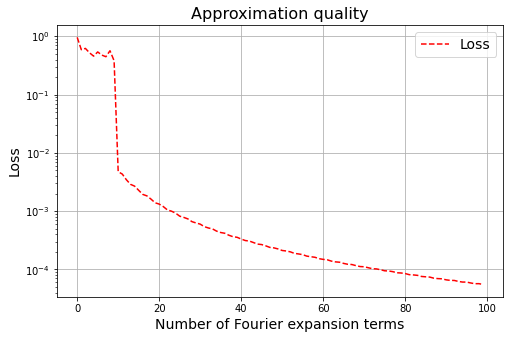
\includegraphics[width=0.65 \textwidth]{images/chapter2/fourier_quality.png}
	\caption{Illustration of the theorems \ref{convergence-l2-norm}, \ref{convergence-pointwise} for the function from the previous example}
	\label{fig:fourier_quality}
\end{figure}